%! Author = choct155
%! Date = 6/22/21

% Preamble
\documentclass[10pt]{article}

% Packages
\usepackage{amsmath, amssymb}
\usepackage{xcolor}
\usepackage{hyperref}
\usepackage{enumitem}
\usepackage{marginnote}
\usepackage{float}
\usepackage{graphicx}
\graphicspath{ {./img/} }
\usepackage [english]{babel}
\usepackage [autostyle, english = american]{csquotes}
\MakeOuterQuote{"}

\definecolor{linkcolor}{HTML}{2d4887}
\definecolor{highlight}{HTML}{c46200}
\hypersetup{
    colorlinks=true,
    urlcolor=linkcolor,
}

% Document
\begin{document}
    \title{Fundamental of Matrix Computation: Section 1.2}
    \author{Marvin Ward jr.}
    \maketitle

    \section{Exercise 1.2.4}
    Prove that \begin{math}A^{-1}\end{math} exists, there can be no nonzero \emph{y} for which \begin{math}Ay=0
    \end{math}.

    \noindent\makebox[\linewidth]{\rule{\textwidth}{0.2pt}}

    \begin{align}
        A y &= 0 \\
        A^{-1} A y &= A^{-1} 0 \\
        y &= 0
    \end{align}


    \section{Exercise 1.2.5}
    Prove that if \begin{math}A^{-1}\end{math} exists, then \begin{math} \text{det}(A) \neq 0\end{math}.

    \noindent\makebox[\linewidth]{\rule{\textwidth}{0.2pt}} \\

    First, we know that \begin{math} \text{det}(AB) = \text{det}(A) \text{det}(B)\end{math} and
    \begin{math} A^{-1} A = I\end{math}.

    \begin{align}
        A^{-1} A &= I \\
        \text{det}(A^{-1}) \text{det}(A) &= \text{det}(I)
    \end{align}

    If \begin{math}\text{det}(A) = 0\end{math}, then \begin{math}\text{det}(A^{-1}) \text{det}(A) = 0\end{math}. But,
    \begin{math}\text{det}(A^{-1}) \text{det}(A) \neq 0\end{math}, it equals the determinant of the identity matrix which
    is a hypercube of volume 1.

    \section{Exercise 1.2.6}
    Identify the system of equations that enables us to determine the voltages at each node.

    \begin{figure}[H]
        \centerline{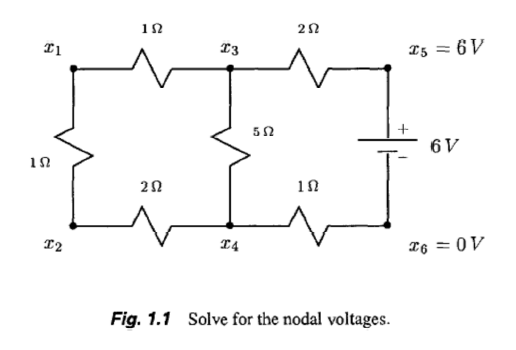
\includegraphics[width=\textwidth]{fig_1_1_circuit}}
        \label{fig:circuit1}
    \end{figure}

    For \begin{math} x_1 \end{math}:
    \begin{align}
        x_1 - x_3 &= 1I_3 \\
        I_3 &= x_1 - x_3 \\
        \dots \\
        x_1 - x_2 &= 1I_2 \\
        I_2 &= x_1 - x_2 \\
        \dots \\
        I_2 + I_3 &= 0 \\
        x_1 - x_2 + x_1 - x_3 &= 0 \\
        2x_1 - x_2 - x_3 &= 0
    \end{align}

    For \begin{math} x_2 \end{math}:
    \begin{align}
        x_2 - x_1 &= 1I_1 \\
        I_1 &= x_2 - x_1 \\
        \dots \\
        x_2 - x_4 &= 2I_4 \\
        I_4 &= 0.5(x_2 - x_4) \\
        \dots \\
        I_1 + I_4 &= 0 \\
        x_2 - x_1 + 0.5(x_2 - x_4) &= 0 \\
        -x_1 + 1.5 x_2 - 0.5x_4 &= 0
    \end{align}

    For \begin{math} x_3 \end{math}:
    \begin{align}
        x_3 - x_1 &= 1I_1 \\
        I_1 &= x_3 - x_1 \\
        \dots \\
        x_3 - x_4 &= 5I_4 \\
        I_4 &= 0.2(x_3 - x_4) \\
        \dots \\
        x_3 - x_5 = x_3 - 6 &= 2I_5 \\
        I_5 &= 0.5(x_3 - 6) \\
        \dots \\
        I_1 + I_4 + I_5 &= 0 \\
        x_3 - x_1 +  0.2(x_3 - x_4) + 0.5(x_3 - 6) &= 0 \\
        -x_1 + 1.7x_3 - 0.2x_4 &= 3
    \end{align}

    For \begin{math} x_4 \end{math}:
    \begin{align}
        x_4 - x_2 &= 2I_2 \\
        I_2 &= 0.5(x_4 - x_2) \\
        \dots \\
        x_4 - x_3 &= 5I_4 \\
        I_3 &= 0.2(x_4 - x_3) \\
        \dots \\
        x_4 - x_6 = x_4 - 0 &= I_6 \\
        I_6 &= x_4 - 0) \\
        \dots \\
        I_2 + I_3 + I_6 &= 0 \\
        0.5(x_4 - x_2) +  0.2(x_4 - x_3) + x_4 &= 0 \\
        -0.5x_2 - 0.2x_3 + 1.7x_4 &= 0
    \end{align}

    All of these manipulations resolve to the following system:

    \begin{equation}
        \begin{bmatrix}
            2 & -1 & -1 & 0 \\
            -1 & 1.5 & 0 & -0.5 \\
            -1 & 0 & 1.7 & -0.2 \\
            0 & -0.5 & -0.2 & 1.7
        \end{bmatrix}
        \begin{bmatrix}
            x_1 \\ x_2 \\ x_3 \\ x_4
        \end{bmatrix} =
        \begin{bmatrix}
            0 \\ 0 \\ 3 \\ 0
        \end{bmatrix}
        \label{eq:circuit_1_system}
    \end{equation}
\end{document}